\documentclass{book}

\usepackage{amssymb}
\usepackage{amsmath}
\usepackage{amsthm}
\usepackage{arydshln}
\usepackage{calc}
\usepackage{cancel}
\usepackage{caption}
\usepackage{cite}
\usepackage{color}
\usepackage{enumitem}
\usepackage{esint}
\usepackage{etoolbox}
\usepackage{float}
\usepackage{framed}
\usepackage{fullpage}
\usepackage{gensymb}
\usepackage[margin=1in]{geometry}
\usepackage{graphicx}
\usepackage{listings}
\usepackage{multirow}
\usepackage{subfiles}
\usepackage{rsfso}
\usepackage{tikz}
\usepackage{tikz-3dplot}
\usepackage{ushort}
\usepackage{wrapfig}
\usepackage{xcolor}
\usepackage{soul}
\usepackage{epstopdf}

% pdf versions
\pdfoptionpdfminorversion=7

% handle page stretching
\raggedbottom

% Graphics file location
\graphicspath{{Graphics/}{../Graphics/}}

% Use for drawings
\usetikzlibrary{angles,arrows,calc,decorations,intersections,patterns,positioning,quotes,shapes}
\usetikzlibrary{shapes.geometric}
\newcommand{\midarrow}{\tikz \draw[-latex] (0,0) -- +(.1,0);}

% Tikz commands for drawing block diagrams, etc...
\tikzset{%
	block/.style    = {draw, rectangle, minimum height = 2em, minimum width = 2em},
	sum/.style      = {draw, circle}, % Adder
	input/.style    = {fill=white, rectangle}, % Input
	output/.style   = {fill=white, rectangle}, % Output
	waypoint/.style   = {coordinate}, % Output
}

\tikzset{%
	startstop/.style= {draw, rectangle, rounded corners, minimum width=2cm, minimum height=1cm,text centered},
	inout/.style    = {draw, trapezium, trapezium left angle=70, trapezium right angle=110, minimum width=2cm, minimum height=1cm, text centered},
	process/.style  = {draw, rectangle, minimum width=2cm, minimum height=1cm, text centered},
	decision/.style = {draw, diamond, minimum width=1.5cm, minimum height=1cm, text centered, diamond, aspect=2},
	arrow/.style    = {thick,-latex,>=stealth},		
}

\tikzset{
	saveuse path/.code 2 args={
		\pgfkeysalso{#1/.style={insert path={#2}}}%
		\global\expandafter\let\csname pgfk@\pgfkeyscurrentpath/.@cmd\expandafter\endcsname
		% not optimal as it is now global through out the document
		\csname pgfk@\pgfkeyscurrentpath/.@cmd\endcsname
		\pgfkeysalso{#1}},
	/pgf/math set seed/.code=\pgfmathsetseed{#1}}

% Define Laplace, Fourier transform symbols
\newcommand{\LT}{\mathcal{L}}
\newcommand{\FT}{\mathcal{F}}

% Define adjugate function
\newcommand{\adj}{\text{adj}}

% Define rank function
\newcommand{\rank}{\text{rank}}

% commands to speed up writing j\omega and s-plane
\newcommand{\jw}{j\omega}
\newcommand{\spl}{s\textrm{-plane}}
% Clean up overline/underline for math mode
\def\obar#1{\bar{#1}}
\def\ubar#1{\ushort{#1}}

\newcommand{\exmp}{\subsubsection*{Example}}
\newcommand{\nib}{\noindent$ \bullet\ $}


\begin{document}
	\chapter*{Lecture 12}
	Last lecture: Control system design via root locus for proportional control.
	
	\noindent Today: Continue discussion of control system design
	\begin{itemize}
		\item Integral control
		\item Derivative control
	\end{itemize}

\section*{Last Lecture}
Recall the system from the previous lecture:
\begin{center}
	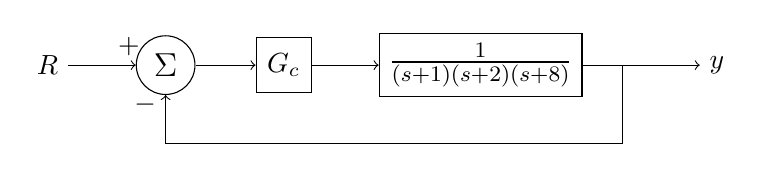
\begin{tikzpicture}[node distance = 1.5cm]
	\node[input] (r) at (0,0) {$ R $};
	\node[sum,right of=r] (sum) {\large$ \Sigma $};
	\node[block, right of=sum] (gc) {$ G_c $};
	\node[block, right of=gc,node distance = 2.5cm] (gp) {\large$ \frac{1}{(s+1)(s+2)(s+8)}$};
	\node[waypoint,below of=gp,node distance = 1cm] (wp) {};
	\node[output, right of=gp,node distance = 3cm] (y) {$ y $};
	\draw[->] (r) -- node[above,pos=0.9] {$ + $} (sum);
	\draw[->] (sum) -- (gc);
	\draw[->] (gc) -- (gp);
	\draw[->] (gp) -- (y);
	\draw[->] ($(gp)!0.6!(y)$) |- (wp) -| node[left,pos=0.9] {$ - $} (sum);
	\end{tikzpicture}
\end{center}
We designed a proportional controller $ G_c=K_p $ so that a unit step input at $ r(t) $ lead to a $ y(t) $ response that met the following requirements:
\begin{enumerate}
	\item overshoot $ \leq 20\% $
	\item peak time $ \leq 2 $ seconds
	\item steady-state error $ \leq $ 0.4
\end{enumerate}
Our design process was as follows:
\begin{enumerate}
	\item Sketch the root locus
	\item From the overshoot requirement, find the minimum damping: $ \zeta \geq 0.46 $
	\item From the peak time requirement, find the minimum natural frequency: $ \omega_n > 1.76 $
	\item Plot the circle for $ \omega_n = 1.76 $ and the line for $ \zeta = 0.46 $ and find where the intercept the root locus
	\item Use the magnitude criterion to find the limiting gains: $ \zeta \geq 0.46 \Rightarrow K_p\leq 38$, $ \omega_n > 1.76 \Rightarrow K_p\geq9 $.
	\item From the the steady-state error requirement, find $ K_p\geq24 $. Therefore, $ 24 \leq K_p\leq 38 $.
	\item Pick a $ K_p $ in that range.
	\item Verify the second-order approximation.
	\item Validate with simulation.
\end{enumerate}

\section*{Integral Control -- Example 2}
Let us consider the same system, but with new performance requriements.
\begin{center}
	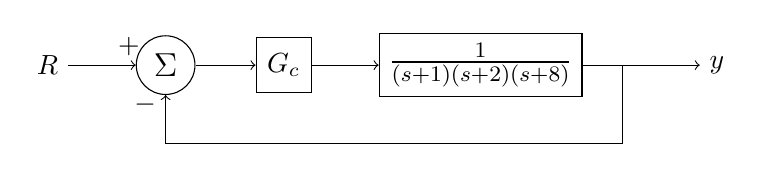
\begin{tikzpicture}[node distance = 1.5cm]
	\node[input] (r) at (0,0) {$ R $};
	\node[sum,right of=r] (sum) {\large$ \Sigma $};
	\node[block, right of=sum] (gc) {$ G_c $};
	\node[block, right of=gc,node distance = 2.5cm] (gp) {\large$ \frac{1}{(s+1)(s+2)(s+8)}$};
	\node[waypoint,below of=gp,node distance = 1cm] (wp) {};
	\node[output, right of=gp,node distance = 3cm] (y) {$ y $};
	\draw[->] (r) -- node[above,pos=0.9] {$ + $} (sum);
	\draw[->] (sum) -- (gc);
	\draw[->] (gc) -- (gp);
	\draw[->] (gp) -- (y);
	\draw[->] ($(gp)!0.6!(y)$) |- (wp) -| node[left,pos=0.9] {$ - $} (sum);
	\end{tikzpicture}
\end{center}
\begin{enumerate}
	\item overshoot $ \leq 20\% $
	\item peak time $ \leq 2 $ seconds
	\item steady-state error $ \leq $ 0.15 (previously 0.4)
\end{enumerate}

Let's start by trying a proportional controller $ G_c = K_p $ again. Following the same procedure as last time, we have $ 9 \leq K_p\leq 38 $ from the overshoot and peak time requirements, and will now look at steady-state error. For a step input:
\[ e_{ss} = \frac{1}{1+\lim_{s\to0}G} \]
\[ e_{ss} = \frac{1}{1+\lim_{s\to0}\frac{K_p}{(s+1)(s+2)(s+8)}} = \frac{1}{1+\frac{K_p}{16}} = \frac{16}{16+K_p} \]
\[ e_{ss} \leq 0.15 \quad\Rightarrow\quad K_p \geq 90.7 \]
This means we must have $ K_p\leq 38 $ to meet the overshoot requirement but $ K_p\geq 90.7 $ to meet the steady-state error. Proportional control will not work! We need a more complicated controller.

How can we reduce $ e_{ss} $?
\begin{itemize}
	\item If our controller has an integrator ($ 1/s $), we will have a Type-1 system, therefore $ e_{ss}=0 $ for a step input.
	\item $ G_c = K_p/s $ will eliminated steady-state error but will introduce its own problems
	\begin{itemize}
		\item Changes shape of root locus.
		\item In this example, it would make meeting the peak time and overshoot requirements impossible.
	\end{itemize}
	\item Can we add something else to $ G_c $ that will minimize the effect of this pole on transient behavior?
	\item We could add a zero just to the left of the origin. Then, the root locus would be mostly unaffected.
	\begin{align*}
	\textrm{PI Control: } G_c = K_p + \frac{K_i}{s} = \frac{K_p s + K_i}{s} = \frac{K(s+z_c)}{s},\quad z\textrm{ is near }0
	\end{align*}
\end{itemize}

\begin{center}
	\begin{tikzpicture}[scale=.75]
	\draw (-10,0) -- (2,0);
	\draw (0,-2) -- (0,2);
	\foreach \x in {-9,-8,-7,-6,-5,-4,-3,-2,-1,0,1} \draw (\x cm,2pt) -- (\x cm,-2pt);
	\node at (0,0) {\Large$ \times $};
	\node at (-0.2,0) {\Large$ \circ $};
	\draw[dashed] (-0.1,0) circle (0.5);
	\node at (-1,0) {\Large$ \times $};
	\node at (-2,0) {\Large$ \times $};
	\node at (-8,0) {\Large$ \times $};
	\draw[thick] (-1,0.01) -- (-2,0.01);
	\draw[thick] (-8,0.01) -- (-10,0.01);
	\draw[thick] (0,0.01) -- (-0.2,0.01);
	%	\draw[thick] (-1.5,0) arc (180:150:3);
	%	\draw[thick] (-1.5,0) arc (180:210:3);
	%	\draw[dashed] (-0.845,-2) -- (-2,0) -- (-0.845,2);
	\end{tikzpicture}
\end{center}

Let's take a closed look at poles and zeros in PI control: We have an open-loop pole at $ s=0 $ and an open-loop zero at $ s=-z_c $, where $ z_c $ is near zero.
\begin{itemize}
	\item If there is no other pole or zero between $ s=0 $ and $ s=z_c $, then they will cancel each other out with respect to the root locus.
	\item The root locus shape (angle criterion) and gains (magnitude criterion) remain the same as for proportional control
\end{itemize} 
For our plant $ \frac{1}{(s+1)(s+2)(s+8)} $, this means we could keep the controller gain the same as in proportional control ($ 24 \leq K\leq 38 $, let's say $ K=30 $) while eliminating steady-state error with a integrator/zero pair (for example, we will place the pole at $ s=-0.1 $). Then,
\[ G_c = \frac{30(s+0.1)}{s} \]
will meet the design requirements. This is called \textbf{PI Control}.

Now, we will use Matlab to compare the root locus of P, I, and PI controllers, and plot a step response for $ K=30 $.

\begin{center}
	\includegraphics[width=0.49\textwidth,trim={1cm 0 1cm 0},clip]{Lecture12Example2Proportional.eps}
	\hfill
	\includegraphics[width=0.49\textwidth,trim={1cm 0 1cm 0},clip]{Lecture12Example2Integral.eps}
	
	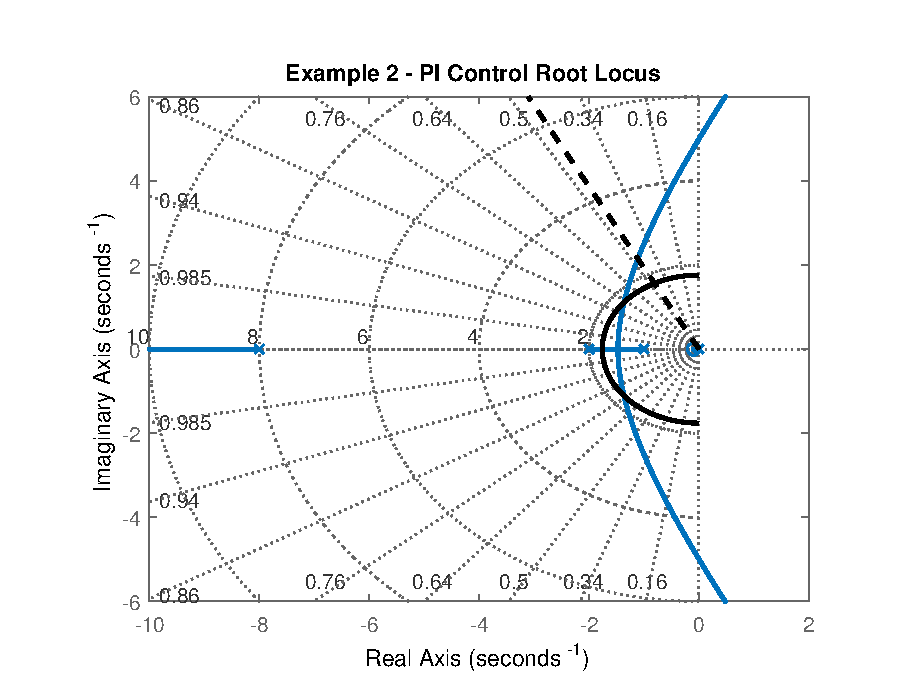
\includegraphics[width=0.6\textwidth]{Lecture12Example2PI.eps}
\end{center}
The proportional control root locus is the same as we found last lecture. Integral control is unable to meet the design requirements: gains that meet the peak time requirements must be outside the $ \omega_n>1.76 $ circle --- this never occurs while the closed-loop system is stable. PI control preserves the root locus of the proportional control system, but also eliminates steady-state error.

\begin{center}
	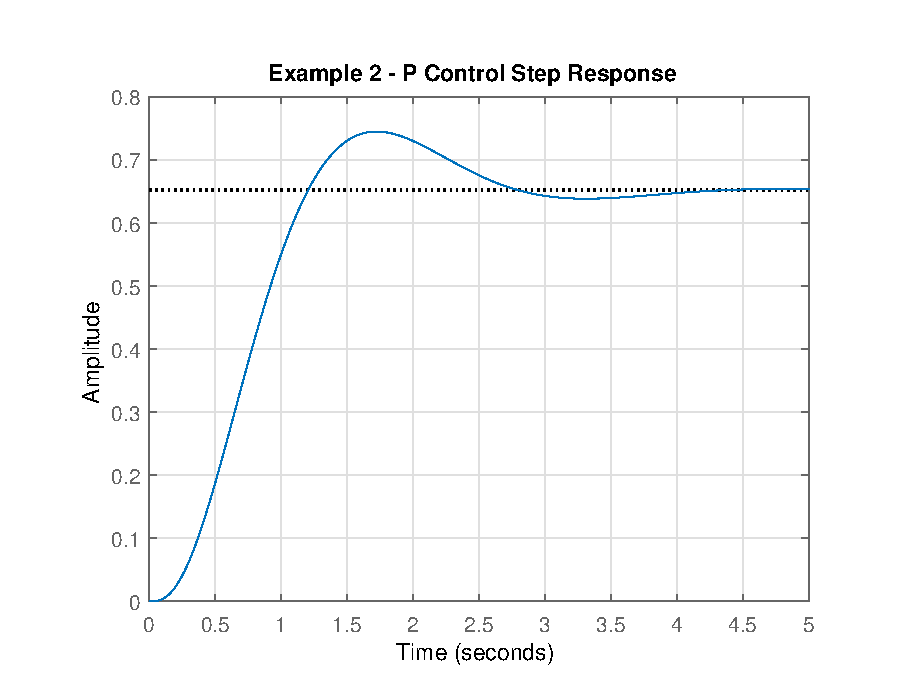
\includegraphics[width=0.49\textwidth,trim={1cm 0 1cm 0},clip]{Lecture12Example2PStep.eps}
	\hfill
	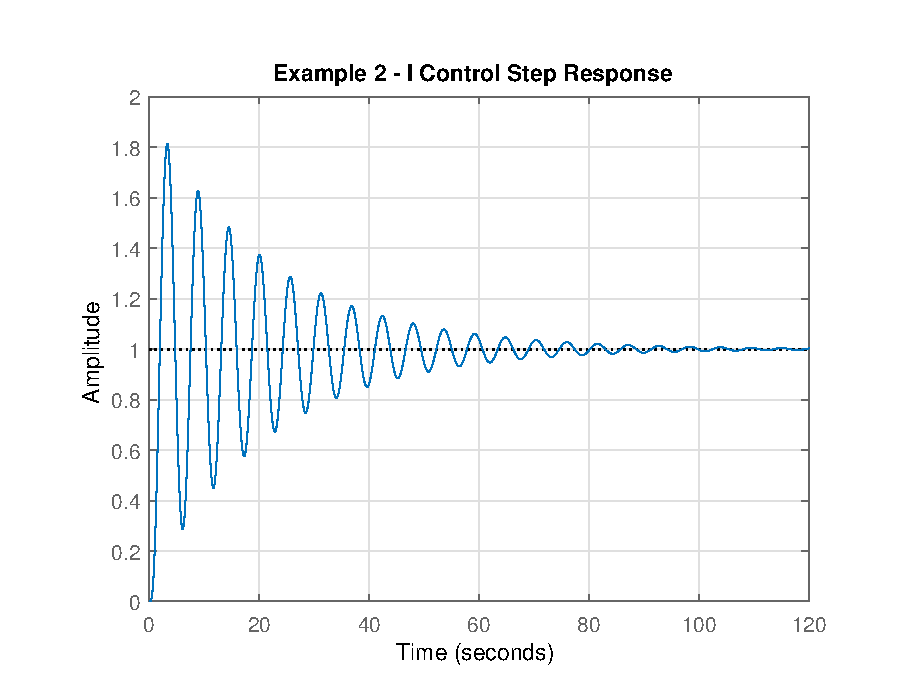
\includegraphics[width=0.49\textwidth,trim={1cm 0 1cm 0},clip]{Lecture12Example2IStep.eps}
	
	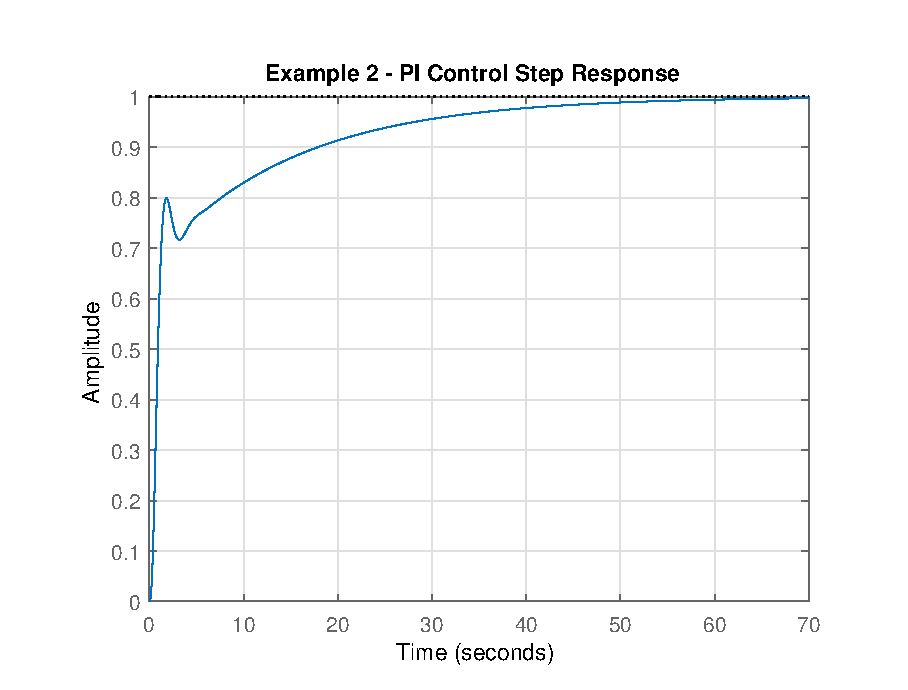
\includegraphics[width=0.6\textwidth]{Lecture12Example2PIStep.eps}
\end{center}

\clearpage
\section*{Derivative Control -- Example 3}
Let us consider the same system, again with new performance requirements.
\begin{center}
	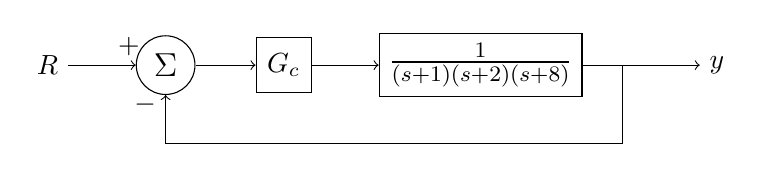
\begin{tikzpicture}[node distance = 1.5cm]
	\node[input] (r) at (0,0) {$ R $};
	\node[sum,right of=r] (sum) {\large$ \Sigma $};
	\node[block, right of=sum] (gc) {$ G_c $};
	\node[block, right of=gc,node distance = 2.5cm] (gp) {\large$ \frac{1}{(s+1)(s+2)(s+8)}$};
	\node[waypoint,below of=gp,node distance = 1cm] (wp) {};
	\node[output, right of=gp,node distance = 3cm] (y) {$ y $};
	\draw[->] (r) -- node[above,pos=0.9] {$ + $} (sum);
	\draw[->] (sum) -- (gc);
	\draw[->] (gc) -- (gp);
	\draw[->] (gp) -- (y);
	\draw[->] ($(gp)!0.6!(y)$) |- (wp) -| node[left,pos=0.9] {$ - $} (sum);
	\end{tikzpicture}
\end{center}
\begin{enumerate}
	\item overshoot $ \leq 20\% $
	\item peak time $ \leq 1.3 $ seconds (previously 2)
	\item steady-state error $ \leq $ 0.4
\end{enumerate}
We will attempt to find a controller using proportional control.

From the first example:
\[ O.S. \leq 20\% \Rightarrow \zeta \geq 0.46 \]
\[ t_p = \frac{\pi}{\omega_n\sqrt{1-\zeta^2}}\Rightarrow\omega_n\geq 2.7 \]
We can plot the root locus and graphically find the gain requirements.

\begin{center}
	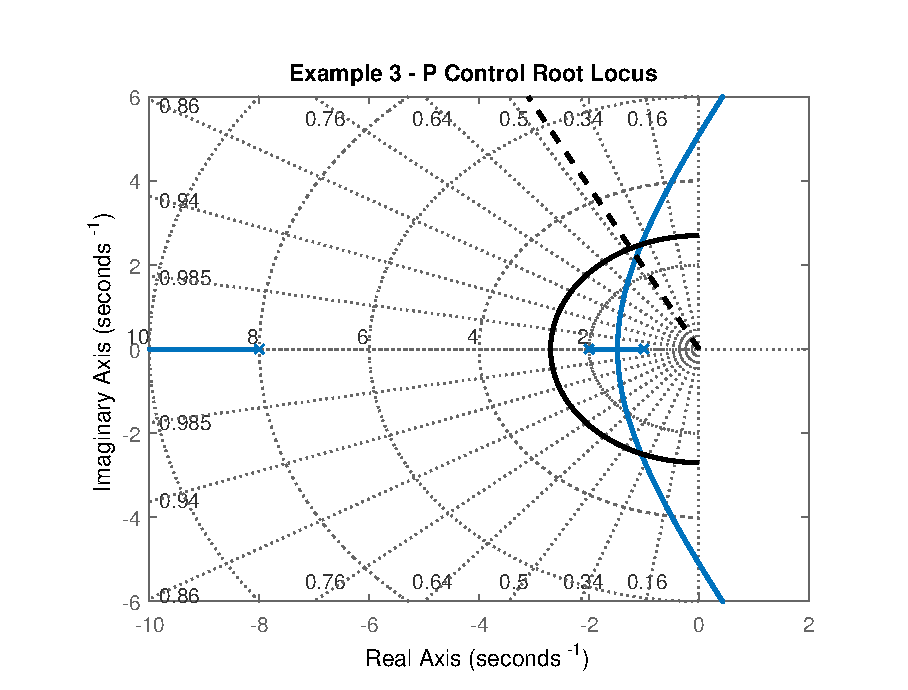
\includegraphics[width=0.5\textwidth]{Lecture12Example3Proportional.eps}
\end{center}
We need to find a point on the root locus that is outside the $ \omega_n\geq2.7 $ circle and below the $ \zeta=0.46 $ line. Clearly, this is not possible. Proportional control will not work for these requirements.

What other options do we have? Let's start with proportional control and add a zero to change the shape of the root locus.
\[ \textrm{PD Control: } G_c = K_p + K_ds = K_d\left(s+\frac{K_p}{K_d}\right) = K_d(s+z_c \]
Note that this transfer function is improper --- we would need to implement a fast pole to make it proper, but at this point don't worry about it.

The method for determining the PD zero location is as follows:
\begin{itemize}
	\item Choose a point you want the root locus to pass though.
	\item Use the angle criterion to find the zero location that makes it possible.
\end{itemize}

For this example, we will find a zero location that let's us place a closed-loop pole at $ s=-1.3\pm2.6j $. This would give us $ \zeta = 0.46 $ and $ \omega_n = 2.9 $, meeting our design requirements. (dobule check all math)

\begin{center}
	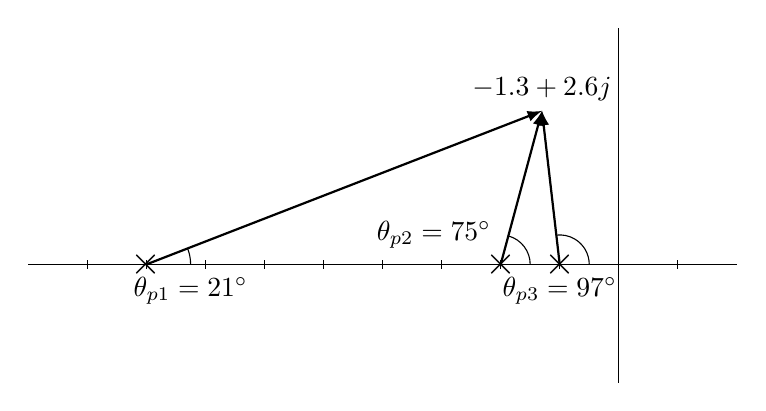
\begin{tikzpicture}[scale=.75]
	\draw (-10,0) -- (2,0);
	\draw (0,-2) -- (0,4);
	\foreach \x in {-9,-8,-7,-6,-5,-4,-3,-2,-1,0,1} \draw (\x cm,2pt) -- (\x cm,-2pt);
	\node at (-1,0) {\Large$ \times $};
	\node at (-2,0) {\Large$ \times $};
	\node at (-8,0) {\Large$ \times $};
	\draw[thick,-latex] (-1,0) -- (-1.3,2.6) node[above] {$ -1.3+2.6j $};
	\draw[thick,-latex] (-8,0) -- (-1.3,2.6);
	\draw[thick,-latex] (-2,0) -- (-1.3,2.6);
	\draw (-0.5,0) arc (0:97:0.5);
	\draw (-1.5,0) arc (0:75:0.5);
	\draw (-7.25,0) arc (0:21:0.75);
	\node[below] at (-7.25,-0.05) {$ \theta_{p1}=21^\circ $};
	\node[left] at (-2,0.5) {$ \theta_{p2}=75^\circ $};
	\node[below] at (-1,-0.05) {$ \theta_{p3}=97^\circ $};
	%	\draw[dashed] (-0.845,-2) -- (-2,0) -- (-0.845,2);
	\end{tikzpicture}
\end{center}
Angle criterion:
\[ \sum \theta_{zi} - \sum \theta_{pi} = 180^\circ \pm \ell 360^\circ \]
\[ \theta_z - 21^\circ - 75^\circ - 97^\circ = 180^\circ \pm \ell 360^\circ \]
\[ \theta_z = 373^\circ \pm \ell 360^\circ = 13^\circ \]
So, if $ \theta_z=13^\circ $, then
\[ \tan(\theta_z) = \tan(13^\circ) = \frac{2.6}{z-1.3} \]
\textit{(Reminder: tangent = opposite over adjacent.)}

Therefore, $ z=12.5 $; a zero is at $ s=-12.5 $ will make the root locus pass through $ 1.3+2.6j $. In addition, our 2nd-order approximation will still be valid.

Next, we can use the magnitude criterion to find the appropriate gain.
\[ K = \frac{M_{p1}M_{p2}M_{p3}}{M_{z}}=\frac{(7.2)(2.7)(2.6)}{11.6} = 4.4 \]
\[ \Rightarrow\quad G_c = 4.4(s+12.5) \]

We can now verify the steady-state error requirement:
\[ e_{ss} = \frac{1}{1+\lim_{s\to0}\frac{4.4(s+12.5)}{(s+1)(s+2)(s+8)}} = \frac{1}{1+\frac{55}{16}} \]
\[ e_{ss} = 0.23 \]

We can then validate with simulation (plots on next page).

\paragraph*{Key Point:} Derivative control is used to modify the root locus. Integral control does not modify the root locus, it only decreases the error.

\begin{center}
	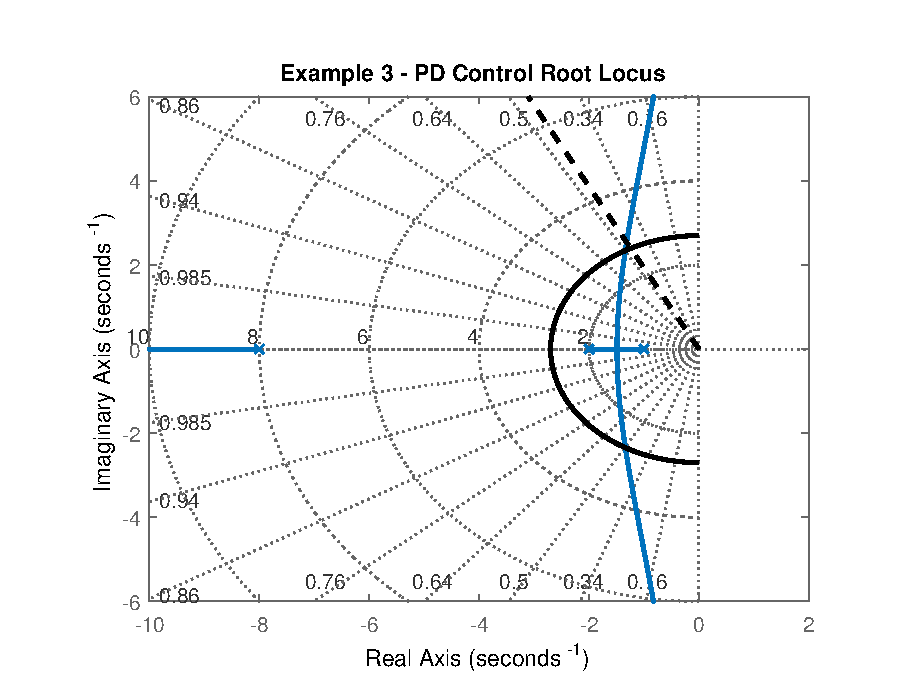
\includegraphics[width=0.49\textwidth,trim={1cm 0 1cm 0},clip]{Lecture12Example3PD.eps}
	\hfill
	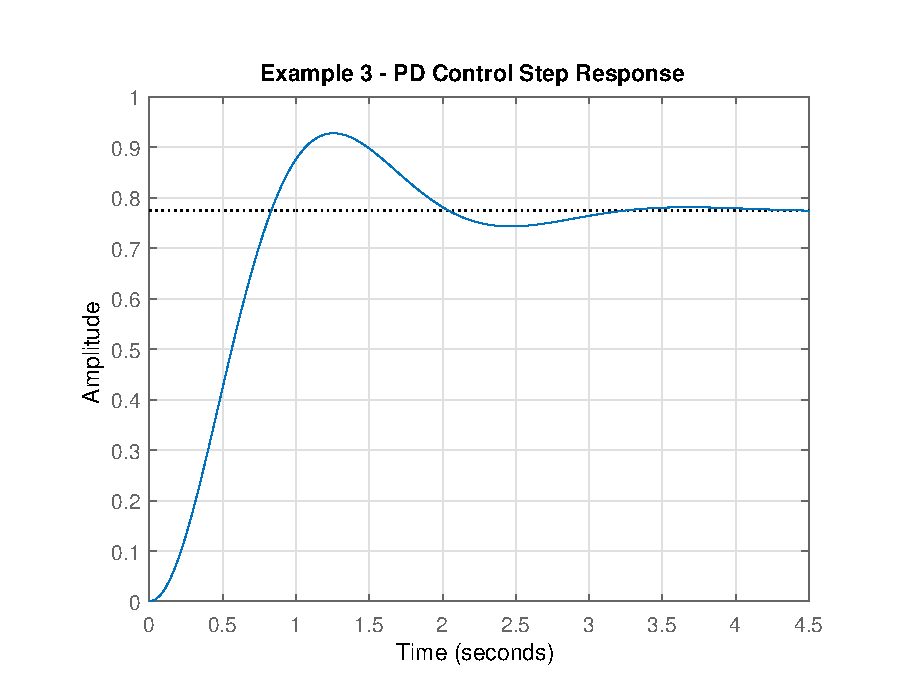
\includegraphics[width=0.49\textwidth,trim={1cm 0 1cm 0},clip]{Lecture12Example3PDStep.eps}
\end{center}

\section*{PID Control -- Example 4}
Let us consider the same system, again with even more restrictive performance requirements.
\begin{center}
	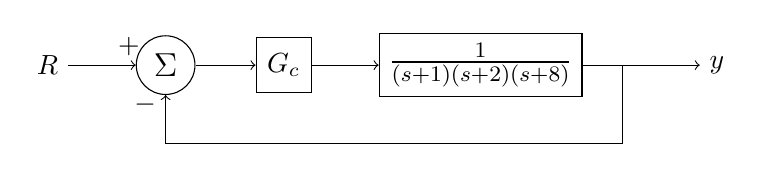
\begin{tikzpicture}[node distance = 1.5cm]
	\node[input] (r) at (0,0) {$ R $};
	\node[sum,right of=r] (sum) {\large$ \Sigma $};
	\node[block, right of=sum] (gc) {$ G_c $};
	\node[block, right of=gc,node distance = 2.5cm] (gp) {\large$ \frac{1}{(s+1)(s+2)(s+8)}$};
	\node[waypoint,below of=gp,node distance = 1cm] (wp) {};
	\node[output, right of=gp,node distance = 3cm] (y) {$ y $};
	\draw[->] (r) -- node[above,pos=0.9] {$ + $} (sum);
	\draw[->] (sum) -- (gc);
	\draw[->] (gc) -- (gp);
	\draw[->] (gp) -- (y);
	\draw[->] ($(gp)!0.6!(y)$) |- (wp) -| node[left,pos=0.9] {$ - $} (sum);
	\end{tikzpicture}
\end{center}
\begin{enumerate}
	\item overshoot $ \leq 20\% $
	\item peak time $ \leq 1.3 $ seconds (previously 2)
	\item steady-state error $ \leq $ 0.05 (previously 0.4)
\end{enumerate}
To meet these requirements, we are going to take our PD controller from the last example ad add integral control. Then,
\[ \text{PID Control: } G_c = K_p + \frac{K_i}{s} + K_d s = \frac{K_d\left(s^2 + \frac{K_p}{K_d}s + \frac{K_i}{K_d}\right)}{s} =  \frac{K_d(s+z_1)(s+z_2)}{s} \]
$ z_1 $ will be chosen to shape the root locus (as in PD control), while $ z_2 $ will be placed near zero to cancel the effects of the integrator on the root locus (as in PI control). Then, we can tune the gain $ K_d $.

Using the gains and zero locations from the previous examples, we have:
\[ G_c = \frac{4.4(s+12.5)(s+0.1)}{s} \]
Is the second-order approximation valid here?

\nib Yes -- the zero at $ -12.5 $ is far enough left to be non-dominant, and the pole and zero near the origin cancel each other.

The root locus and step response of this system are shown below.
\begin{center}
	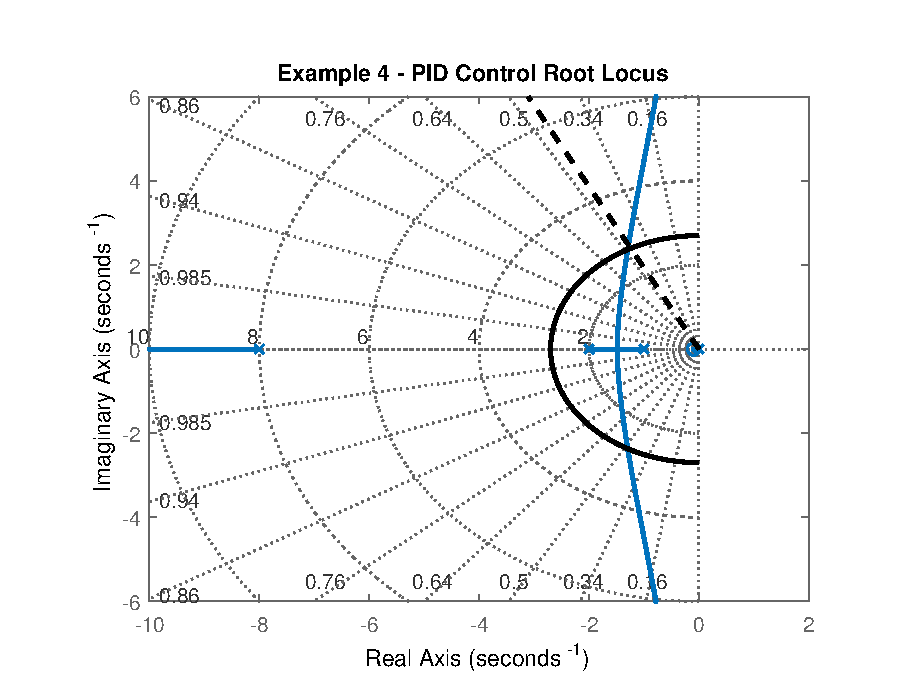
\includegraphics[width=0.49\textwidth,trim={1cm 0 1cm 0},clip]{Lecture12Example4PID.eps}
	\hfill
	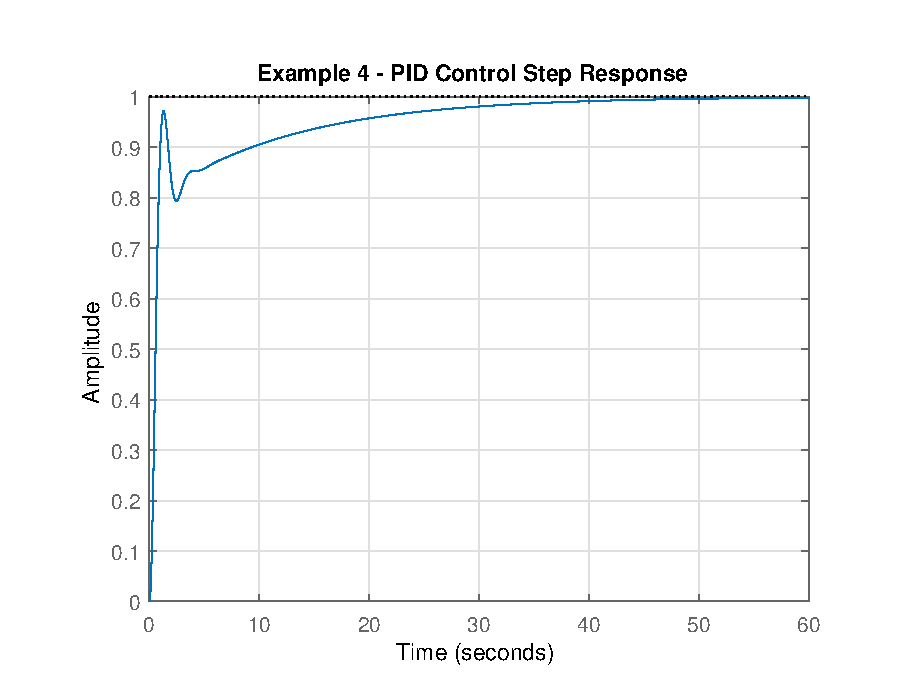
\includegraphics[width=0.49\textwidth,trim={1cm 0 1cm 0},clip]{Lecture12Example4PIDStep.eps}
\end{center}

The following procedure can be used for root locus controller design:
\begin{center}
	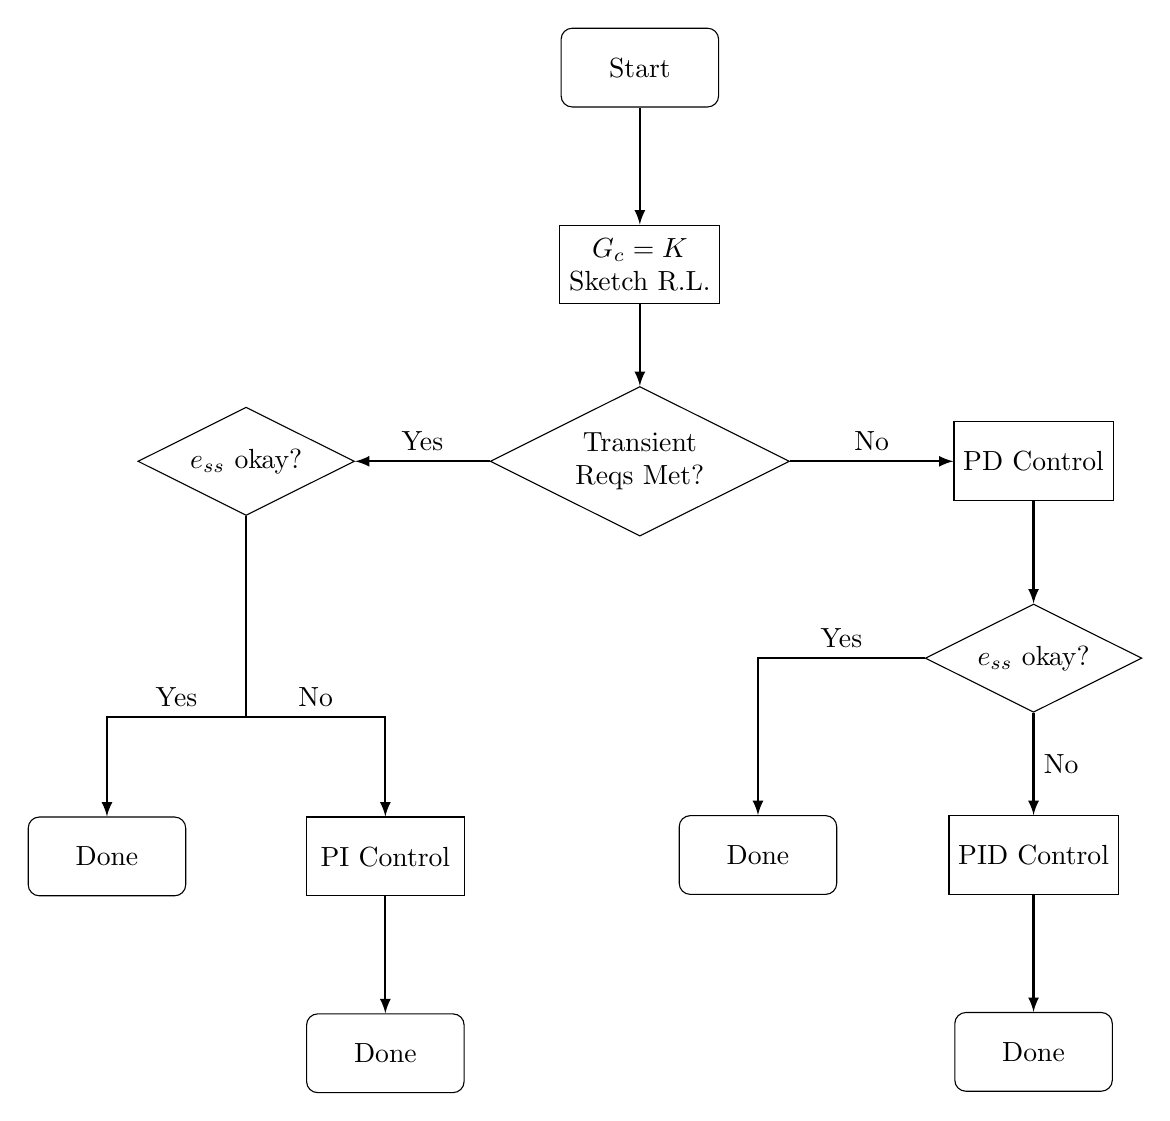
\begin{tikzpicture}[node distance=2.5cm]
	\node[startstop] (start) {Start};
	\node[process, below of=start,align=center] (P) {$ G_c = K $\\Sketch R.L.};
	\node[decision, below of=P,align=center] (Req1) {Transient\\Reqs Met?};
	\node[decision, left of=Req1,node distance=5cm] (CheckEssP) {$ e_{ss} $ okay?};
	\node[waypoint,below of=CheckEssP,node distance = 3.25cm] (wpPI) {};
	\node[process, below right of=wpPI] (PI) {PI Control};
	\node[startstop,below left of=wpPI] (PDone) {Done};
	\node[startstop,below of=PI] (PIDone) {Done};
	\node[process, right of=Req1,node distance=5cm] (PD) {PD Control};
	\node[decision, below of=PD] (CheckEssPD) {$ e_{ss} $ okay?};
	\node[process, below of=CheckEssPD] (PID) {PID Control};
	\node[startstop,left of=PID,node distance = 3.5cm] (PDDone) {Done};
	\node[startstop,below of=PID] (PIDDone) {Done};
	
	\draw[arrow] (start) -- (P);
	\draw[arrow] (P) -- (Req1);
	\draw[arrow] (Req1) -- node[above] {Yes} (CheckEssP);
	\draw[arrow] (CheckEssP) -- (wpPI) -| node[above,pos=0.25] {Yes} (PDone);
	\draw[arrow] (CheckEssP) --  (wpPI) -| node[above,pos=0.25] {No} (PI);
	\draw[arrow] (PI) -- (PIDone);
	\draw[arrow] (Req1) -- node[above] {No} (PD);
	\draw[arrow] (PD) -- (CheckEssPD);
	\draw[arrow] (CheckEssPD) -| node[above,pos=0.25] {Yes} (PDDone);
	\draw[arrow] (CheckEssPD) -- node[right] {No} (PID);
	\draw[arrow] (PID) -- (PIDDone);
	\end{tikzpicture}
\end{center}



\section*{Lead/Lag Control}
We will briefly talk about some alternatives to PI, PD, and PID control: Lead, Lag, and Lead/Lag control.
\subsubsection*{Lead Control}
\begin{itemize}
	\item $ \dfrac{s+z_c}{s+p_c} $, $ z_c < p_c $
	\item Lead control is kind of like derivative control.
	\item Place a zero and a pole to the left of the zero to shape the root locus.
	\item Pulls the root locus to the left, but not as much as just a zero at $ s=-z_c $.
	\item PD control reduces the number of asymptotes by 1. Lead control keeps them the same.
\end{itemize}
\begin{center}
	\begin{tikzpicture}[scale=1]
	\draw (-10,0) -- (2,0);
	\draw (0,-1.5) -- (0,1.5);
	\node at (-8,0) {\Large$ \times $};
	\node at (-6.5,0) {\Large$ \circ $};
	\node at (-4,0) {\Large$ \times $};
	\node at (-2,0) {\Large$ \times $};
	\node at (-1,0) {\Large$ \times $};
	\draw[thick,-latex] (-8,0) -- (-10,0);
	\draw[thick,-latex] (-4,0) -- (-6.5,0);
	\draw[thick] (-1,0) -- (-2,0);
	\draw[thick,-latex] (-1.5,0) arc (180:150:3);
	\draw[thick,-latex] (-1.5,0) arc (180:210:3);
	\draw[dashed] (-7.25,0) ellipse (1.25 and 0.5);
	\node[below] at (-7.25,-0.5) {Lead Control};
	\end{tikzpicture}
\end{center}
\subsubsection*{Lag Control}
\begin{itemize}
	\item $ \frac{s+z_c}{s+p_c} $, $ z_c > p_c $
	\item Kind of like integral control.
	\item Place a pole just left of the origin (instead of \textit{at} the origin), and a zero to the left of the pole. 
	\item The pole and zero would still cancel each other out with respect to transient behavior.
	\item Does not effect root locus (pole and zero cancel).
	\item Reduces $ e_{ss} $, but does not increase system type (i.e., can't reduce $ e_{ss} $ to zero).
	\item The state-state error will be less than for proportional control, but this may be okay based on design requirements. 
	\item A large ratio of $ z_c/p_c $ will reduce error the most, which is accomplished by moving $ p_c $ near the origin (while keeping $ z_c $ close).
\end{itemize}
\begin{center}
	\begin{tikzpicture}[scale=1]
	\draw (-7,0) -- (2,0);
	\draw (0,-1.5) -- (0,1.5);
	\node at (-0.2,0) {\Large$ \times $};
	\node at (-0.5,0) {\Large$ \circ $};
	\node at (-5,0) {\Large$ \times $};
	\node at (-3,0) {\Large$ \times $};
	\node at (-2,0) {\Large$ \times $};
	\draw[thick,-latex] (-0.2,0) -- (-0.4,0);
	\draw[thick,-latex] (-5,0) -- (-7,0);
	\draw[thick] (-2,0) -- (-3,0);
	\draw[thick,-latex] (-2.5,0) arc (180:150:3);
	\draw[thick,-latex] (-2.5,0) arc (180:210:3);
	\draw[dashed] (-0.35,0) ellipse (0.5 and 0.25);
	\node[below right] at (0,0) {Lag Control};
	\end{tikzpicture}
\end{center}
\exmp
Compare the steady-state error for a step input for the two systems:
\begin{center}
	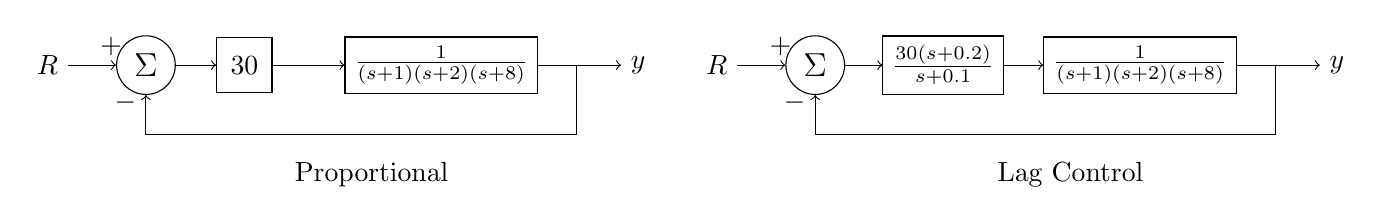
\begin{tikzpicture}[node distance = 1.25cm]
	\node[input] (r) at (0,0) {$ R $};
	\node[sum,right of=r] (sum) {\large$ \Sigma $};
	\node[block, right of=sum] (gc) {$ 30 $};
	\node[block, right of=gc,node distance = 2.5cm] (gp) {$ \frac{1}{(s+1)(s+2)(s+8)} $};
	\node[waypoint,below left of=gp,node distance = 1.25cm] (h) {};
	\node[output, right of=gp,node distance = 2.5cm] (y) {$ y $};
	\draw[->] (r) -- node[above,pos=0.9] {$ + $} (sum);
	\draw[->] (sum) -- (gc);
	\draw[->] (gc) -- (gp);
	\draw[->] (gp) -- (y);
	\draw ($(gp)!0.6875!(y)$) |- (h);
	\draw[->] (h) -| node[left,pos=0.9] {$ - $} (sum);
	\node[below of=h,node distance=0.5cm] {Proportional};
	
	\node[input] (r2) at (8.5,0) {$ R $};
	\node[sum,right of=r2] (sum2) {\large$ \Sigma $};
	\node[block, right of=sum2,node distance = 1.625cm] (gc2) {$ \frac{30(s+0.2)}{s+0.1} $};
	\node[block, right of=gc2,node distance = 2.5cm] (gp2) {$ \frac{1}{(s+1)(s+2)(s+8)} $};
	\node[waypoint,below left of=gp2,node distance = 1.25cm] (h2) {};
	\node[output, right of=gp2,node distance = 2.5cm] (y2) {$ y $};
	\draw[->] (r2) -- node[above,pos=0.9] {$ + $} (sum2);
	\draw[->] (sum2) -- (gc2);
	\draw[->] (gc2) -- (gp2);
	\draw[->] (gp2) -- (y2);
	\draw ($(gp2)!0.6875!(y2)$) |- (h2);
	\draw[->] (h2) -| node[left,pos=0.9] {$ - $} (sum2);
	\node[below of=h2,node distance=0.5cm] {Lag Control};
	\end{tikzpicture}
\end{center}
For a Type-0 system, $ e_{ss} = \frac{1}{1+\lim_{s\to 0}G} $.
\[\text{Proportional: } e_{ss} = \frac{1}{1 + \lim_{s\to 0} \frac{30}{(s+1)(s+2)(s+8)}} = \frac{1}{1+\frac{30}{16}}=0.35 \]
\[\text{Lag Control: } e_{ss} = \frac{1}{1 + \lim_{s\to 0} \frac{30(s+0.2)}{(s+0.1)(s+1)(s+2)(s+8)}} = \frac{1}{1+\frac{6}{1.6}}=0.21 \]
So, lag control reduces the steady-state error (but does not bring it to zero).
\subsubsection*{Lead/Lag Control}
We can combine lead control and lag control to get ``lead/lag'' control, similar to how we combined PD and PI control to get PID control.
\section*{Final Comments on Controller Design}
\begin{itemize}
	\item P, PI, PD, and PID controllers work well for many applications and are widely used.
	\item There are not the only types of controller possible.
	\item If you have a system where the 2nd order approximation is \textbf{not} valid, our design process won't work right.
	\item But, our knowledge of what closed-loop pole locations mean is still valid:
	\begin{itemize}
		\item All poles in LHP $ \to $ stable system
		\item Poles on real axis $ \to $ no overshoot
		\item Closed-loop zero near closed-loop pole $ \to $ cancellation
		\item Poles farther left $ \to $ faster transient behavior
	\end{itemize}
\end{itemize}

\end{document}
